\documentclass[12pt]{article}
\usepackage[utf8]{inputenc}
\usepackage{geometry}
\usepackage{xcolor}
\usepackage{tcolorbox}
\usepackage{titlesec}
\usepackage{graphicx}

\geometry{top=2cm, bottom=2cm, left=2.5cm, right=2.5cm}

\definecolor{promptbg}{rgb}{0.92, 0.95, 0.98}
\definecolor{promptborder}{rgb}{0.2, 0.4, 0.8}

\renewcommand{\normalsize}{\fontsize{13.5}{16.5}\selectfont}
\renewcommand{\large}{\fontsize{15}{18}\selectfont}
\renewcommand{\Large}{\fontsize{17}{20}\selectfont}
\renewcommand{\LARGE}{\fontsize{21}{25}\selectfont}

\titleformat{\section}{\Large\bfseries\centering}{}{0em}{}
\titleformat{\subsection}{\large\bfseries\centering}{}{0em}{}
\titleformat{\subsubsection}{\normalsize\bfseries\centering}{}{0em}{}

\renewcommand{\familydefault}{\sfdefault}

\begin{document}

\begin{flushright}
\large
Gabriela Mora, V-31.541.893 \\
Lucía Martínez, V-31.906.577 \\
Maivet Pereira, V-30.814.708 \\
\end{flushright}

\vspace{0.4cm}

\begin{center}
    {\LARGE \textbf{Evaluación del Recurso de Ayuda para el Simulador de Caché de Correspondencia Directa y Asociativa por Vías}} \\[0.3cm]
    \large Arquitectura del Computador \\[0.2cm]
    \large 1 de Septiembre de 2026
\end{center}

\vspace{0.4cm}

\section*{Recurso original}

La infografía de referencia del proyecto 1 es un material de apoyo claro y bien estructurado que cubre los conceptos fundamentales para un simulador de caché:

\begin{itemize}
    \item Decodificación de direcciones (Tag, Index, Offset).
    \item Implementación base con estructuras de datos (\texttt{std::vector} y \texttt{std::list}).
    \item Estrategias de optimización como el prefetch.
    \item Tabla comparativa de políticas de ubicación.
\end{itemize}

El recurso cumple su propósito y fue de utilidad durante el desarrollo del proyecto.

\section*{Validación del Recurso de Ayuda}

El recurso fue validado durante la implementación del simulador. Ayudó a comprender:

\begin{itemize}
    \item La división de la dirección en Tag, Index y Offset.
    \item La diferencia entre mapeo directo, asociativo por vías y totalmente asociativo.
    \item La utilidad del prefetch para reducir fallos.
\end{itemize}

\section*{Propuesta de Mejora}

Complementamos el recurso añadiendo tres aspectos clave de nuestra implementación:

\begin{itemize}
    \item \textbf{Matriz con \texttt{vector<vector<lineaCache>>}:} A diferencia del recurso original que usaba \texttt{list} (acceso secuencial), nosotros optamos por una matriz de \texttt{vector} para acceder directamente a cualquier línea por su índice, haciendo el simulador más rápido y eficiente O(1).
    \item \textbf{LRU con contador \texttt{ultimoUso}:} Lo implementamos así porque es más sencillo: solo actualizamos un número en cada acceso y reemplazamos el más antiguo.
    \item \textbf{Diagrama de flujo del proceso de lectura:} Incluimos un diagrama que muestra paso a paso el flujo completo, especialmente cómo actúa el prefetch.
\end{itemize}

Estas mejoras reflejan cómo adaptamos el recurso a nuestra implementación práctica en C++, manteniendo la esencia del contenido original pero aportando una visión más cercana a nuestro desarrollo.

\section*{Prompt para la mejora}

\begin{tcolorbox}[
    colback=promptbg,
    colframe=promptborder,
    coltitle=black,
    title=Prompt utilizado,
    sharp corners,
    boxrule=1.2pt,
    left=6pt,
    right=6pt,
    top=4pt,
    bottom=4pt
]
\begin{small}
\begin{verbatim}
"Conservando la esencia de la infografía original e incorporando una nueva paleta 
de colores basada en tonos azules y beige, genera una infografía técnica corta y 
precisa que detalle los componentes internos y el funcionamiento algorítmico de 
un simulador de memoria caché en C++, incluyendo la estructura de datos jerárquica 
con organización asociativa por vías, la decodificación de direcciones de 32 bits, 
el algoritmo de reemplazo LRU y el flujo lógico de operaciones de lectura y 
prefetch."
\end{verbatim}
\end{small}
\end{tcolorbox}

\begin{figure}[!ht]
    \centering
    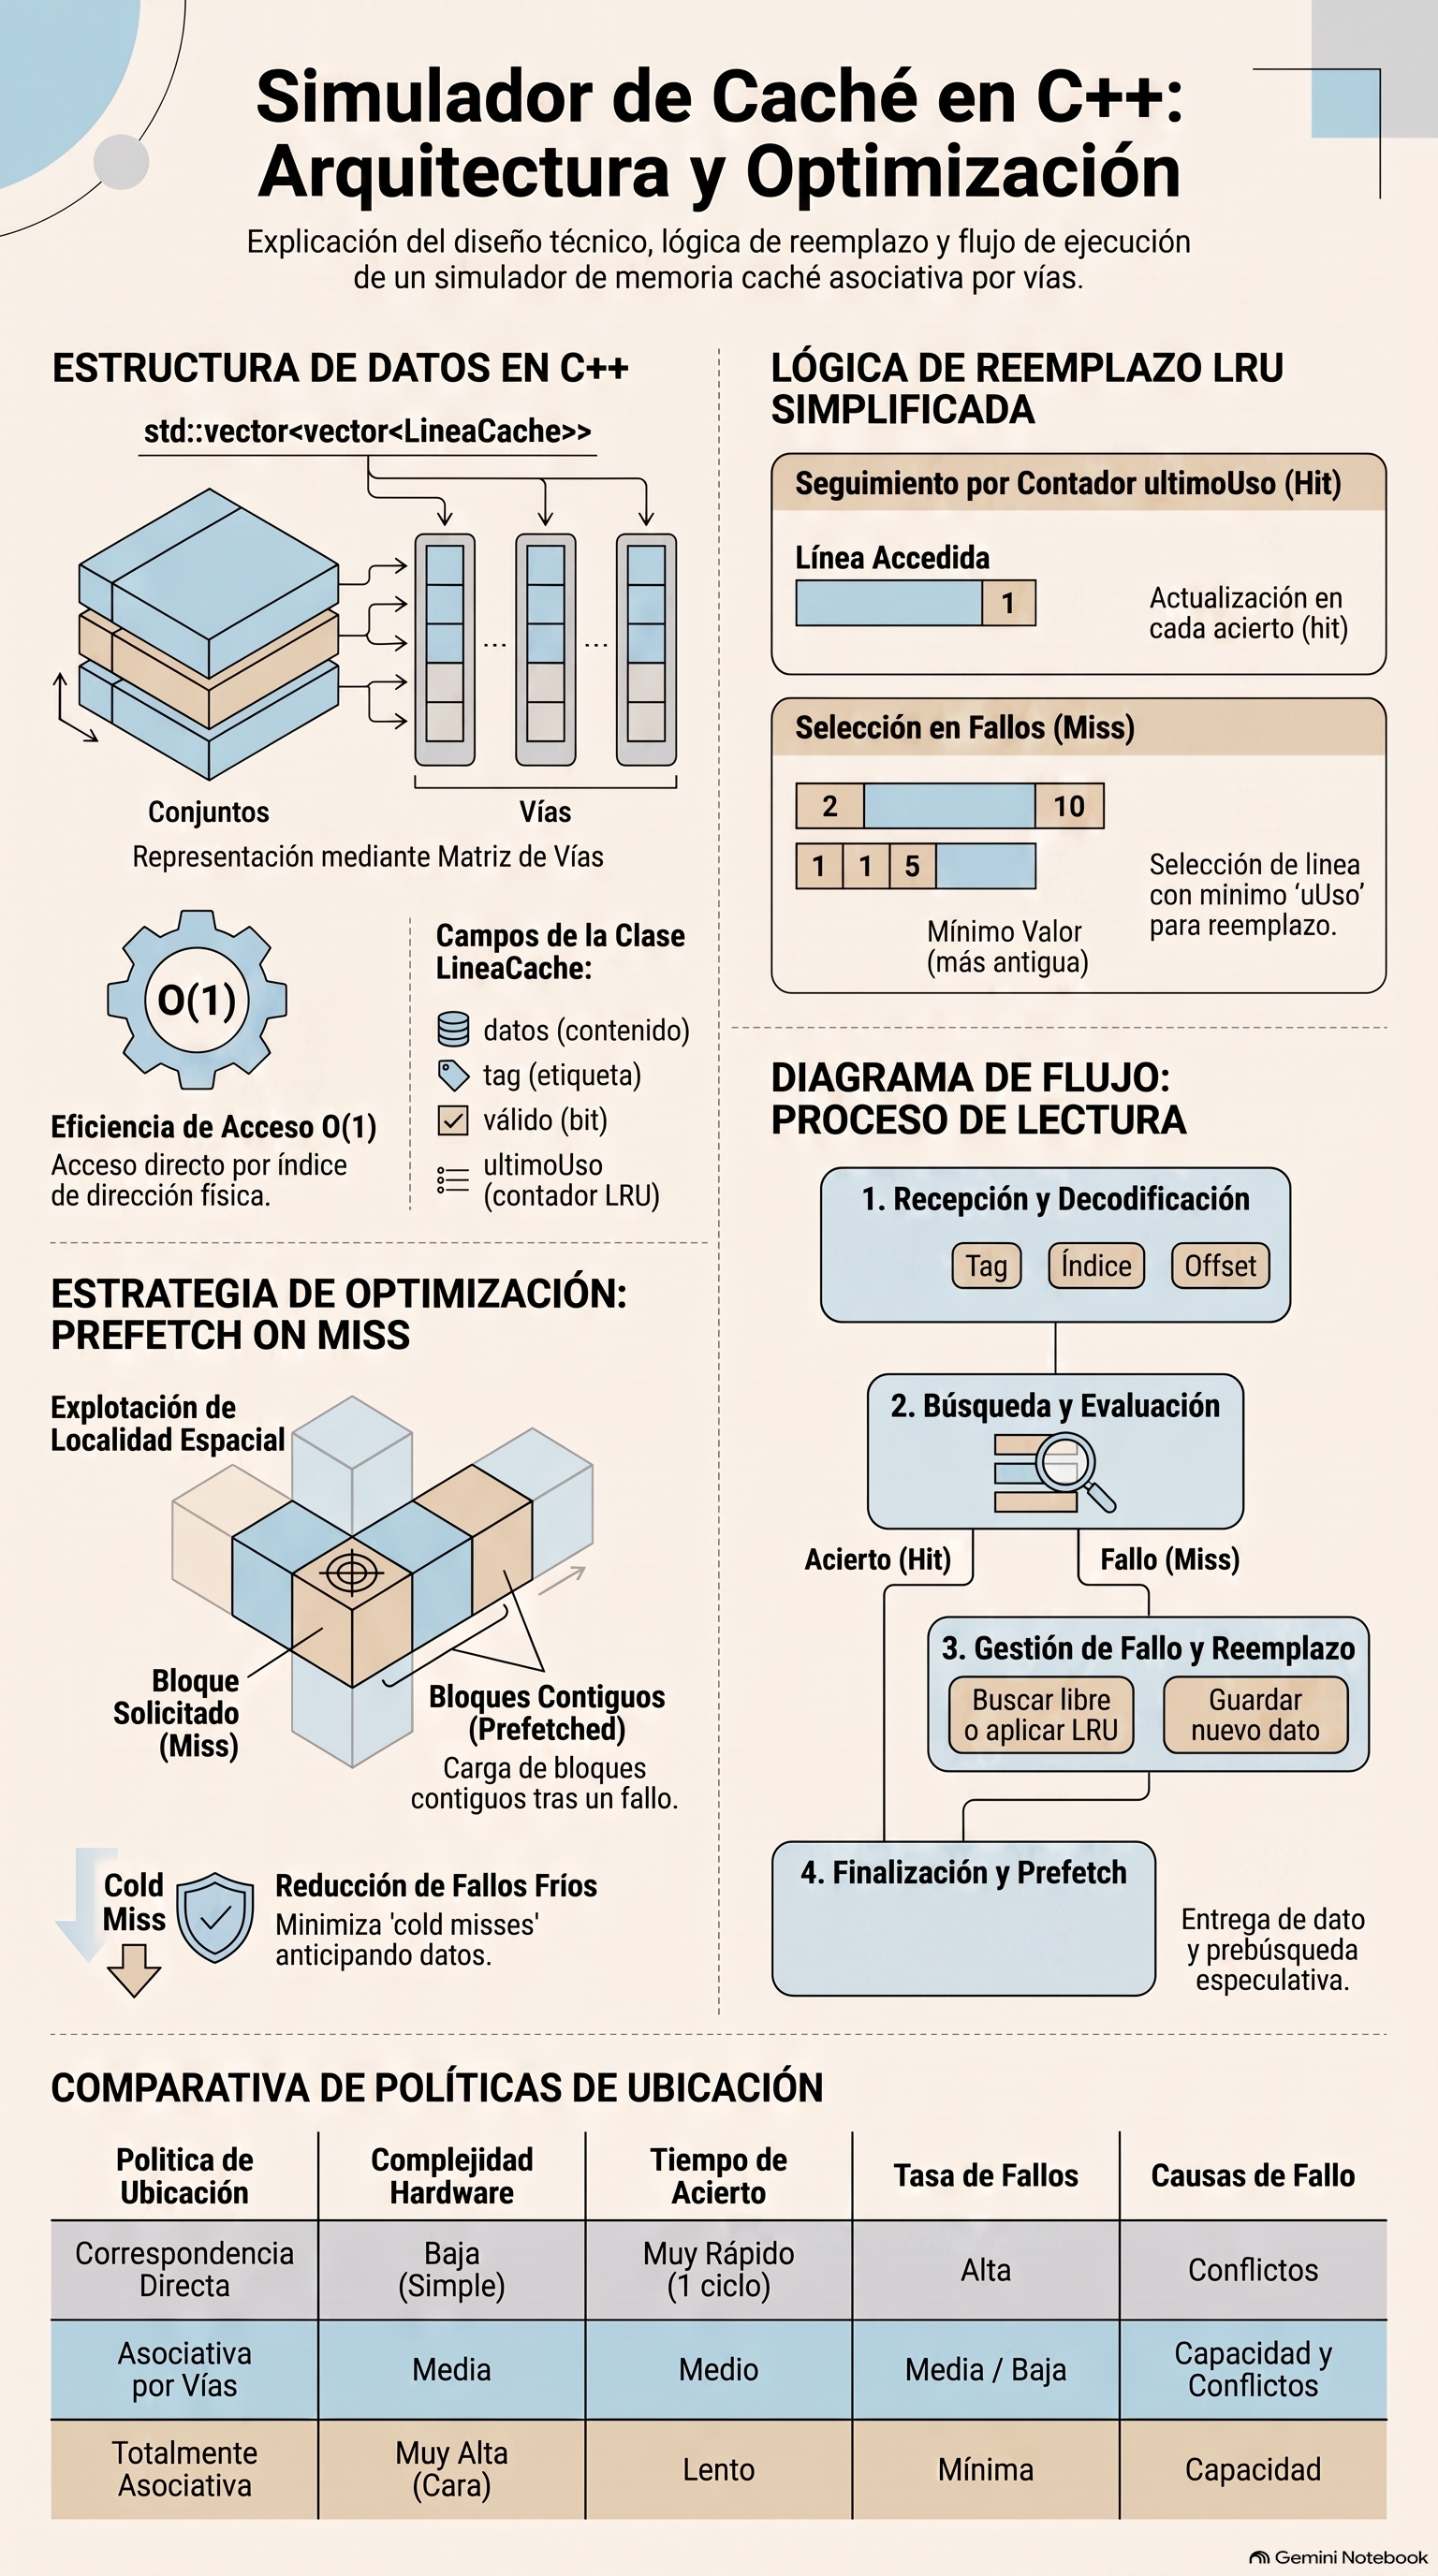
\includegraphics[width=0.75\textwidth, keepaspectratio]{infografia.png}
    \caption{Infografía mejorada}
    \label{fig:infografia}
\end{figure}

\end{document}